\documentclass[twocolumn,11pt]{article}
\setlength{\textheight}{9truein}
\setlength{\topmargin}{-0.9truein}
\setlength{\parindent}{0pt}
\setlength{\parskip}{10pt}
\setlength{\columnsep}{.4in}

\usepackage{amsmath,amsfonts,amssymb,amsthm,bm,caption,calc,ifthen,graphicx,url,hyperref}
\usepackage{pythonhighlight}

\begin{document}
\pagestyle{plain}
\begin{onecolumn}
ASTP720 
\newline Final Project
\newline Will Wainwright
\newline Repository: \href{https://github.com/wjwainwright/ASTP720}{https://github.com/wjwainwright/ASTP720}
\end{onecolumn}
\section*{Introduction}
Object oriented programming is the practice of creating data structures to store information. These data structures have their own associated properties and methods, which allows uniform operations between objects of the same type. In addition to the default objects in python, packages and individuals can create their own objects. 

In some cases, you may wish to have multiple objects that are similar to each other but differ in some ways. In this scenario, it makes sense to make use of object inheritance. Objects that you create can be made as children to a parent class. These child objects will inherit the properties and methods of the parent class, and can add methods in addition that do not appear in the parent class. Child classes can also overwrite methods and properties of their parent classes, including operator overloading. This allows for the creation of a more dynamic system of data structures.

\section*{Discussion}
As an example of object inheritance, I created a galaxy class. This class initializes galaxy objects with a few initial parameters, namely the name of the galaxy and the radius. The galaxy class also has a method to return the density of the galaxy. In the case that the galaxy does not have a determined mass or volume, the method returns None.
\newline
\begin{python}
class galaxy():
    def __init__(self,name,radius):
        self.name = name
        self.radius = radius
        self.mass = None
        self.volume = None
    
    def calcDensity(self):
        try:
            assert not self.mass == None
        except:
            print(f"Mass has not been calculated for {self.name}")
            return
        try:
            assert not self.volume == None
        except:
            print(f"Volume has not been calculated for {self.name}")
            return
        
        self.density = self.mass/self.volume
        return self.density
\end{python}

After creating an initial galaxy class, I created two child classes, the spiral galaxy and elliptical galaxy. In order to assign a parent to these classes, they are created as $class$ $spiralGalaxy(galaxy)$. This lets python know that the $spiralGalaxy$ is a special instance of a $galaxy$. When overwriting the default $\_\_init\_\_$ method, we can call $super().\_\_init\_\_()$ to pass information to the parent's initialization method. The two galaxies have varied methods of detecting the volume and mass, but both make use of the parent's method to calculate density. Finally, I also created a special type of elliptical galaxy, the dwarf spheroidal. These mass and volume of these galaxies is essentially calculated the same way, so no methods need to be overwritten from the elliptical galaxy inherited methods. As such, we can declare the class as a instance of elliptical galaxies and then simply write $pass$. This lets python know that we do not wish to overwrite any inherited methods or add any new ones, and simply to pass everything given to the child object to its parent.
\newline
\begin{python}
class spiralGalaxy(galaxy):
    def __init__(self,name,radius,thickness,vrot,Nspiral):
        super().__init__(name,radius)
        self.thickness = thickness
        self.vrot = vrot
        self.Nspiral = Nspiral
    
    def getNspiral(self):
        return self.Nspiral
    
    def calcMass(self):
        G = 6.67e-11
        
        self.mass = self.vrot**2*self.radius/G
        
        return self.mass
    
    def calcVolume(self):
        import numpy as np
        
        self.volume = np.pi*self.radius**2*self.thickness
        
        return self.volume
\end{python}

Spiral galaxies are created with a name and radius, which is passed to the parent galaxy object. In addition, spiral galaxies have a disk height, or thickness, a rotational velocity, and a number of spiral arms. These properties are stored as parameters of the child and not the parent. The first additional method, $getNspiral()$, is just an example of a getter-setter practice which I usually neglect in Python. It is good security practice to not allow the end user to have direct access to the object variables, and instead have a method for setting a value and a method that returns the value. The spiral galaxy class has its own methods to calculate mass and volume. The volume calculation is based on the geometry of a cylinder, $V=\pi R^2h$. The mass calculation is an estimation of the mass that can be calculated using the radius $R$, the rotational velocity at that radius $v_{rot}(R)$, and the gravitational constant $G$. The equation is therefore $M=\frac{v_{rot}^2R}{G}$. One interesting thing to note about object inheritance is that despite the $calcDensity()$ method being a parent object method, it can still access the child variable for $self.mass$. In order to properly determine the density of a spiral galaxy class object, you must first calculate its mass and volume.
\newpage

\begin{python}
class ellipticalGalaxy(galaxy):
    def __init__(self,name,radius,velocityDispersion,eccentricity,k=3):
        #Note: radius for elliptical is assumed to be semi-major axis length a
        super().__init__(name,radius)
        self.velocityDispersion = velocityDispersion
        self.k = k
        self.eccentricity = eccentricity
    
    def calcMass(self):
        G = 6.67e-11
        
        self.mass = self.k*self.radius*self.velocityDispersion**2/G
        
        return self.mass
    
    
    def calcVolume(self):
        import numpy as np
        
        a = self.radius
        b = self.radius*np.sqrt(1-self.eccentricity**2)
        
        #Compromise between two types of ellipsoid volumes, a^2b and ab^2
        c = (a+b)/2
        
        self.volume = 4/3*np.pi*a*b*c
        
        return self.volume
\end{python}

Much like the spiral galaxy class object, the elliptical galaxy class object has its own mass and volume calculation methods. Elliptical galaxy objects are initialized with a name and radius, which are then passed to the parent galaxy object. In this class, the radius is treated as the semi-major axis, $a$. The elliptical galaxy is also initialized with an eccentricity $e$ and a velocity dispersion $\sigma$. The volume of the elliptical galaxy is calculated as an ellipsoid. Traditionally, an ellipsoid with no symmetries would have the volume of $V=\frac{4}{3}\pi abc$. The semi-minor axis, $b$, can be determined from $b=a\sqrt{1-e^2}$. An oblate ellipsoid would have a value of $c=a$, and a prolate ellipsoid has a value of $c=b$. This makes their volumes $V=\frac{4}{3}\pi a^2b$ and $V=\frac{4}{3}\pi ab^2$ respectively. As a compromise between these two and instead of requiring $c$ to be an initialized variable, I went with an estimate of $c=\frac{a+b}{2}$. While this is not an exact determination of the volume for an elliptical galaxy, I would say it is no less realistic than knowing the values of $a$, $b$, and $c$ for a real galaxy. One way to estimate the mass of an elliptical galaxy is through the equation $M=3\frac{\sigma^2R}{G}$. The value of the coefficient in front of the ratio is often subject to change depending on who you ask, but 3 is a pretty safe approximation and it's what I learned in galactic astrophysics. Once again, the mass and volume must be calculated before calling for the density.

As an attempted application of this data structure, I wanted to be able to map out the densities of the galaxies in a galaxy cluster. A real data set that includes the values specified in my class objects is unlikely, so as a placeholder I have created simulated data. Figure \ref{fig:cluster} shows the placement of these galaxy objects in a box, which represents the cluster. Figure \ref{fig:density} shows the density of these clusters in $mks$. Overall, I would say that the application of these principles could use a bit more work as far as the data simulation goes, as I was only able to use rough estimates for the upper and lower bounds for the given properties of a cluster that I required. Future improvements to the project would involve the determination of mass and volume via different methods. For example, I could pass all known measurements of a galaxy into the initialization. Based on which measurements are available, the object could then `decide' which mass determination method to employ. This would allow for a much more realistic and versatile use case and would not require the creation of a fake data set. However, I would say that the lesson that can be learned about object inheritance and its importance to the broader use of object oriented programming is an important one. I hope that the reader has learned something from this brief topic overview, or at least that it has helped to reinforce understanding of the topic.

\begin{figure}[!h]
	\centering
      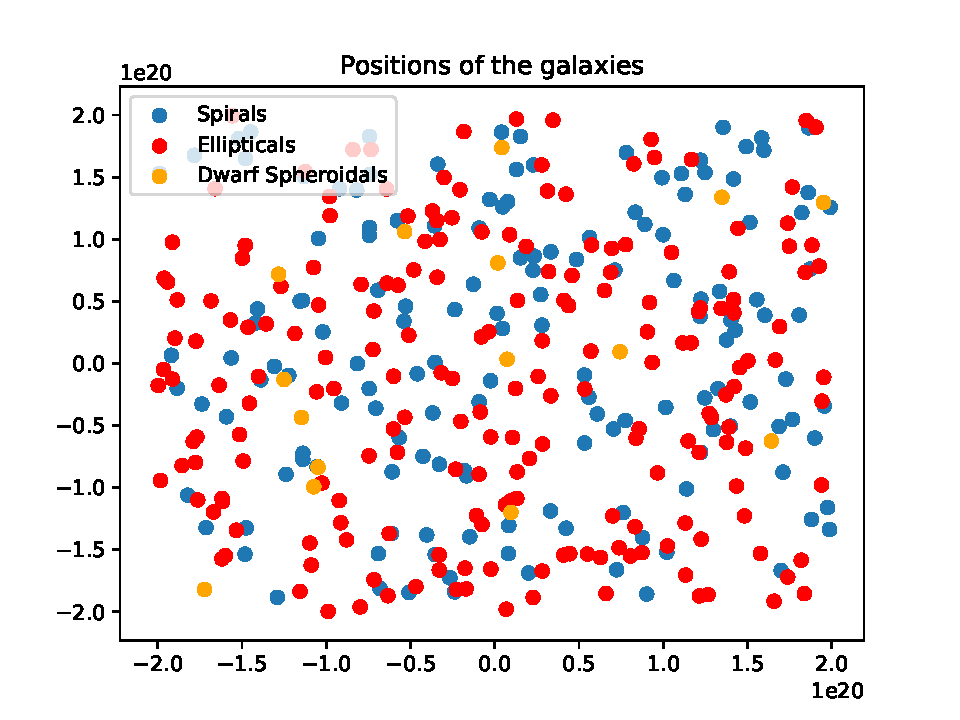
\includegraphics[width=5.5in]{cluster.pdf}
	\caption{}
	\label{fig:cluster}
\end{figure}

\begin{figure}[!h]
	\centering
      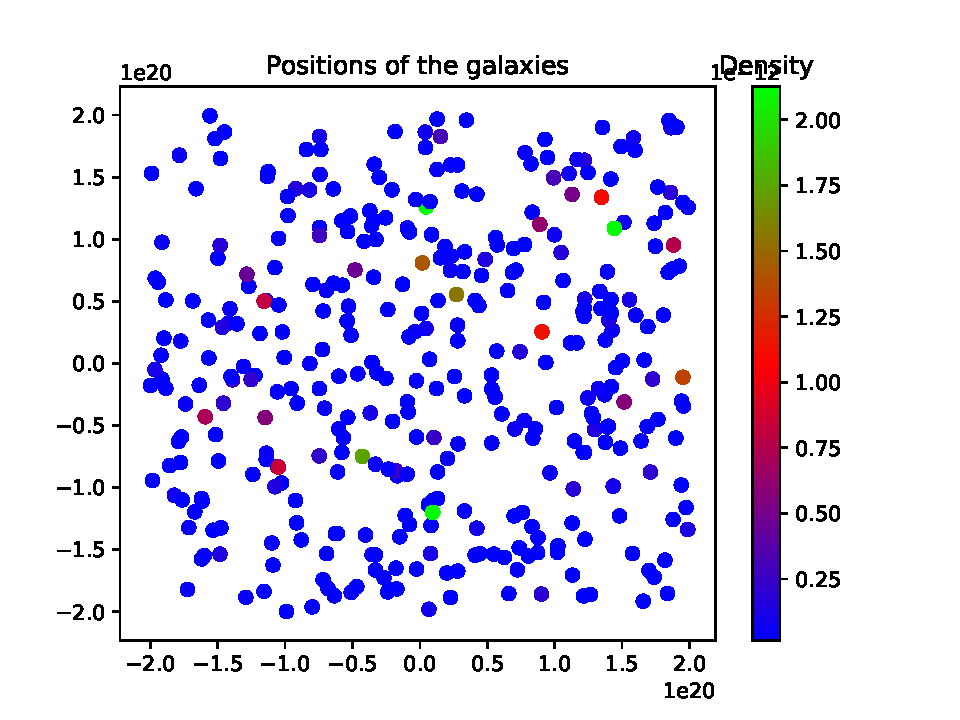
\includegraphics[width=5.5in]{density.pdf}
	\caption{}
	\label{fig:density}
\end{figure}




\end{document}